\documentclass[conference]{IEEEtran}
\IEEEoverridecommandlockouts

\usepackage{cite}
\usepackage{amsmath,amssymb,amsfonts}
\usepackage{algorithmic}
\usepackage{graphicx}
\usepackage{textcomp}
\usepackage{xcolor}
\usepackage{stfloats}
\usepackage{algorithm2e}

\def\BibTeX{{\rm B\kern-.05em{\sc i\kern-.025em b}\kern-.08em
    T\kern-.1667em\lower.7ex\hbox{E}\kern-.125emX}}
\begin{document}

\title{GPS-Free Self-Healing Drone Networks\\via Virtual Spring-Dampers}

\author{
\IEEEauthorblockN{Federico Corò, Riccardo Fabbian, and Claudio E. Palazzi}
\IEEEauthorblockA{\textit{Department of Mathematics} \\
\textit{University of Padua}\\
Padua, Italy \\
federico.coro@unipd.it, fabb.riccardo@gmail.com, cpalazzi@math.unipd.it
}}

\newcommand{\fc}[1]{{\color{red}{FC: #1}}}


\maketitle

\begin{abstract}
Distributed collective intelligence enables groups of autonomous agents to cooperatively achieve system-level goals through local interactions and decentralized decision-making. In this context, this paper presents a self-healing protocol for drone swarms that restores
connectivity to a base station after link loss. The protocol combines ACK-based
reachability detection, flooding-based hop discovery, periodic neighbor
broadcasts, and a virtual spring-damper formation controller. Localization is
GPS-free and uses a UWB PHY-layer channel with anchor beacons, Time-of-Flight
ranging, and least-squares trilateration. We evaluate the system in
\textit{ns-3} on 15 single-base scenarios that vary topology, swarm
density, ranging noise, and scheduled drone failures. The protocol restores
connectivity within $\sim1$\,s in every scenario; between the two
attractive-force variants, healing latency is the same, while the weighted
variant reduces mean return latency by $8\%$ and its $p_{95}$ tail by $21\%$.
\end{abstract}

\begin{IEEEkeywords}
Distributed Collective Intelligence, Drone Swarm, UWB, Trilateration, Localization, Self-Healing.
\end{IEEEkeywords}

\section{Introduction}
%%%Drone swarms provide larger coverage, redundancy, and modular task specialization compared to single drones, but require robust communication between drones and base stations, as well as coordinated formation control~\cite{ouyang2023formation}. In decentralized swarm operations, links between a drone and the base are frequently interrupted by jamming or geographic occlusions. The swarm must then autonomously detect the loss and reorganize through a ``self-healing'' protocol that forms a multi-hop relay chain, avoiding partitioning without centralized control.

Drone swarms represent a compelling instance of distributed collective intelligence, where autonomous agents cooperate through local sensing, communication, and decentralized decision-making to achieve system-level objectives. Compared to single drones, swarms provide larger coverage, redundancy, and modular task specialization, but they also require robust communication between drones and base stations, as well as coordinated formation control~\cite{ouyang2023formation}. In decentralized swarm operations, communication links between individual drones and the base station may be disrupted by jamming, interference, or geographic occlusions. In such situations, the swarm must autonomously detect connectivity loss and collectively reorganize through a self-healing process that restores communication via a multi-hop relay chain, preventing network partitioning without centralized control.

%%%We implement such a protocol in which drones detect loss of base connectivity and reorganize via a virtual spring-damper controller. Localization is GPS-free and is obtained from UWB Time-of-Flight trilateration against fixed anchors. We evaluate two controller variants (centroid and weighted) in \textit{ns-3} on a single-base batch that varies topology, swarm density, ranging noise, and scheduled drone failures. The contributions are: a UWB-based GPS-free communication and localization stack, a self-healing protocol with return and station-keeping behavior, and a comparison of the two controller variants on this batch.

To address this challenge, in this work in progress paper we present and discuss a self-healing protocol in which drones detect the loss of base connectivity and cooperatively reconfigure their positions through a virtual spring-damper controller. Localization is performed without GPS and relies on UWB Time-of-Flight trilateration against fixed anchors. We evaluate two controller variants (centroid and weighted) in \textit{ns-3} on a single-base experimental batch that varies topology, swarm density, ranging noise, and scheduled drone failures. The main contributions of this work are: a UWB-based GPS-free communication and localization stack, a self-healing protocol with return and station-keeping behaviors, and a comparative evaluation of the two controller variants under varying network and environmental conditions.

The rest of this paper is organized as follows. Section~\ref{sec:related-work} provides an overview of the related literature. Section~\ref{sec:self-healing} presents the proposed self-healing solution. In Sections~\ref{sec:exp-setup} we discuss the experimental setup we employed and in Section~\ref{sec:results} we discuss the outcome of our tests. In Section~\ref{sec:future} we propose the next steps of this work-in-progress, while in Section~\ref{sec:conclusions} conclusions are drawn.


\section{Related Work}
\label{sec:related-work}
Restoring connectivity in mobile multi-agent systems has been studied across
several research lines. In wireless sensor and actor networks, topology
management surveys~\cite{younis2014topology} and cascaded-relocation
schemes~\cite{abbasi2009recovering} recover from node failures by triggering
only the minimum number of nodes after a partition. Restore connectivity
through mobile relays~\cite{senel2011optimized} has shown that deploying mobile
actors to bridge disjoint segments is more efficient than complete redeployment,
an insight that motivates self-healing of the relay-chain in aerial settings.

For unmanned aerial vehicles, formation control is based on classical flocking
and potential-field methods. Olfati-Saber's flocking
framework~\cite{olfatisaber2006flocking} and Khatib's artificial potential
fields~\cite{khatib1986real} provide the analytical basis that virtual
spring-damper models~\cite{piemngam2019virtual, chen2015virtual} extend to
networked agents. Real flying swarms have demonstrated decentralized
coordination using only local
communication~\cite{hauert2011reynolds, vasarhelyi2018optimized}, while
Coppola~\textit{et al.}~\cite{coppola2018onboard} showed that 
relative localization based on on-board communication is sufficient for safe MAV teaming.

GPS-free self-localization is a parallel concern. UWB ranging combined with
anchor beacons supports centimeter-level positioning for aerial
robots~\cite{hamer2018selfcalibrating, mai2018local}. Our contribution
integrates these strands by combining UWB-only localization, a hop-aware
spring-damper controller, and an explicit loss-of-link detector to
autonomously restore single-base connectivity after drone failures.

\section{Self-Healing Protocol}
\label{sec:self-healing}
The protocol enables a drone to detect loss of communication with the base
station and autonomously reorganize to form a multi-hop relay chain. It has two components: a loss-of-link detector and a formation controller based on a virtual spring-damper model. Upon ACK timeout, a drone runs the controller using neighbor positions and hop counts (obtained by flooding). The controller produces attractive forces toward the preceding and following hops
in the relay chain, plus repulsive forces against close neighbors. The
equilibrium is the geometric midpoint between the previous and next hop, which maximizes the Signal-to-Noise Ratio on both incident links.
Figure~\ref{fig:scenario} sketches a representative scenario: an in-coverage drone whose direct link is about to fail, and the post-healing relay chain that helper drones form to restore connectivity.

\begin{figure}[t]
    \centering
    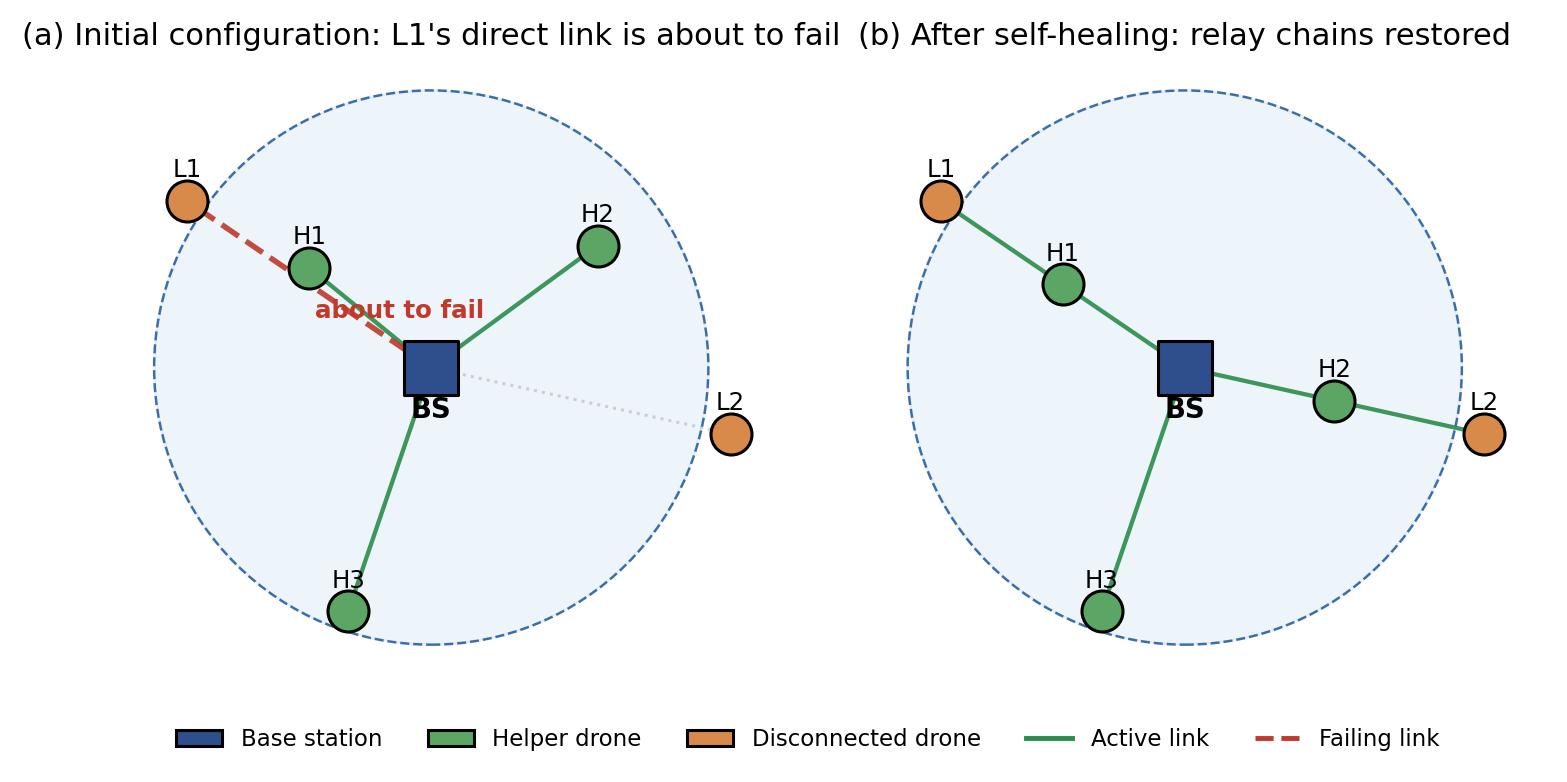
\includegraphics[width=\columnwidth]{scenario_before_after.png}
    \caption{Self-healing scenario. (a) Initial layout: helper drones (H1--H3)
    are inside coverage; L1 holds a direct link to the base that is about to
    fail (red dashed), while L2 is already isolated. (b) After the
    spring-damper repositioning, helpers move outward to bridge each
    disconnected drone with the base via a multi-hop relay.}
    \label{fig:scenario}
\end{figure}

\subsection{System Architecture}
The architecture has three node roles: a stationary Base Station ($B$),
static UWB Anchors ($A_j$), and mobile Drones ($D_i$) running an identical
control stack. The base station also acts as an anchor. Following the
Crazyflie~2.1 model~\cite{bitcraze_crazyflie}, base traffic is unicast while
swarm coordination uses broadcast. Messages are delivered over a UWB
PHY-layer channel that adds propagation delay ($d$/$c$) and enforces a
range cutoff. Each drone dispatches packets to four logical modules:
hop-discovery flooding, a neighbor table keyed by neighbor ID, a UWB
ranging/trilateration module, and core control logic for position updates,
ACKs, and help-proxy requests. The controller reads UWB position and
neighbor data and emits a velocity command through an actuator. The base
station tracks position updates, replies with ACKs (carrying base position
and hop 0), and periodically seeds floods.

\subsection{Help-Proxy Triggering}
Each drone sends periodic unicast \texttt{PositionUpdate} messages to the base
and waits for an ACK. If no ACK arrives within a safety window of $1.5s$, the drone
considers the link broken and broadcasts a ``help-proxy'' signal
(\texttt{HELP\_PROXY} CORE packet); any peer receiving it switches into
mission mode. Broadcast matches the Crazyflie communication model.

After issuing \texttt{HELP\_PROXY}, the requester is return-armed once it
receives the first relayed ACK addressed to itself. Return begins after a
hop-staggered timeout similar to 802.11p, proportional to $(H_{max}-h)$
where $H_{max}$ is max hop distance from any drone back to the base
while $h$ is the drone's own hop count.
This enables the farthest drones return first and propagate a \texttt{RETURNING} flag
back along the chain, collapsing it from the tail inward. During return, the
attractive gain is reduced and the drone moves toward direct coverage; on
receiving a direct ACK it enters station-keeping near the coverage boundary,
re-arming if coverage is lost again to prevent oscillation.

\subsection{Flooding-Based Hop Discovery}
Flooding allows drones to estimate the hop distance to the base station even when
direct connectivity is lost. The base periodically broadcasts a
\texttt{START}; every in-coverage drone becomes an initiator and rebroadcasts
a \texttt{DISCOVERY} with hop~1. Broadcast initiation (instead of unicast to
a chosen seed) avoids relying on a single node that might be out of range. On
\texttt{DISCOVERY} reception, a drone with a live direct ACK declares hop~1;
otherwise it increments the carried hop. A node that detects an ACK timeout
suppresses its stale ``hop~1'' until the next flood, preventing false
attraction toward a dead link. Each node only reacts when a shorter path to 
the base arrives arrives for the same flood instance, then emits a \texttt{REPORT} 
and rebroadcasts \texttt{DISCOVERY}; reports are forwarded at most once per
improvement, keeping the protocol lightweight.

\subsection{Neighbor Information Exchange}
For local, decentralized reactivity, each drone maintains a neighbor table
fed by periodic \texttt{NEIGHBOR} broadcasts. The payload carries the sender
ID, its hop count to the base, and UWB-trilaterated coordinates. When a drone
has a direct ACK from the base, it injects a synthetic neighbor entry for
the base (position from the ACK, hop~0), so the controller can treat the
base as just another neighbor without special-casing.

\subsection{Formation Control via Virtual Spring-Damper Model}
Healing behavior is realized by a virtual spring-damper
controller~\cite{piemngam2019virtual, chen2015virtual} that combines
linear attraction to neighbors at adjacent hop levels (the previous and
next hops in the relay chain) with $1/d^2$ short-range repulsion against any
neighbor closer than the safety distance $D_{safe}$:
\begin{equation}
    \vec{F}_{tot} = \!\!\!\sum_{j \in N_{prev}\cup N_{next}}\!\!\! K_{att}(\vec{p}_j-\vec{p}_i) - \!\!\!\sum_{\substack{j \in N \\ d_{ij} < D_{safe}}}\!\!\! \frac{K_{rep}}{d_{ij}^{\,2}}\cdot\frac{\vec{p}_j-\vec{p}_i}{d_{ij}}
\end{equation}
where $\vec{p}_i$ and $\vec{p}_j$ are the positions of drone $i$ and neighbor $j$; 
$N_{prev}$ and $N_{next}$ are the sets of neighbors at the previous 
and next hop levels (hop $h-1$ and $h+1$); $N$ is the set of all neighbors; 
$d_{ij} = \lVert\vec{p}_i - \vec{p}_j\rVert$ is the Euclidean distance between 
drones; $K_{att}$ and $K_{rep}$ are the attractive and repulsive gains 
(Table~\ref{tab:sim-values}); and $D_{safe}$ is the minimum safe separation distance.
The attractive term drives a drone toward the midpoint of its previous and next 
hops; repulsion is applied to all neighbors, including peers with the same hop count. 
We compare two attractive variants: (i) \textit{centroid} groups neighbors by hop count and
applies one pull per group centroid, while (ii) \textit{weighted} scales each pull
by the opposite-side population so the midpoint stays the equilibrium even
under unbalanced sides. The net force is converted to acceleration via
Newton's second law and applied through a velocity actuator capped at
$V_{max}$. A mission flag gates the controller: drones broadcast neighbor
state while idle and switch on the spring-damper loop when a help-proxy
trigger is received.

\section{Experimental Setup}
\label{sec:exp-setup}
The protocol was evaluated in a custom \textit{ns-3}~\cite{ns3simulator}
scenario built around a direct UWB PHY-layer channel that delivers each
transmission after a $d$/$c$ propagation delay with a strict range cutoff. Static UWB anchors and the base station itself periodically broadcast position-tagged beacons; drones compute Time-of-Flight ranges and estimate their pose by least-squares trilateration. The baseline scenario
uses one base at $(0,0,0)$, 20 drones, and 18 standalone anchors. Six drones act as helpers on a $\sim$40\,m ring just inside the 50\,m coverage radius;
11 drones start in the 68--82\,m belt just outside coverage; three far scouts at 112--118\,m force a multi-hop chain. Anchor placement guarantees
at least three line-of-sight beacons everywhere. Each drone ticks at
0.05\,s, performing a position update to the base, an ACK-timeout check
(with \texttt{HELP\_PROXY} on miss), and a controller step. The ACK
timeout is 1.5\,s, position updates are sent every 0.5\,s or on movement,
and anchors beacon at 2\,Hz. A JSON declaration file runs batches that
override positions and schedule mid-simulation drone failures.
Table~\ref{tab:sim-values} lists the baseline parameters.

\begin{table}[t]
\caption{Baseline Simulation Parameter Values}
\label{tab:sim-values}
\centering
\begin{tabular}{|l|l|}
\hline
\textbf{Parameter} & \textbf{Value} \\ \hline
Coverage radius $R_{max}$ & $50$ m \\ \hline
Coverage area & Circular, centered at base station \\ \hline
Number of drones $N_d$ & $20$ \\ \hline
Number of anchors $N_a$ & $18$ \\ \hline
Controller algorithm & centroid, weighted \\ \hline
Attractive gain $K_{att}$ & $0.3$ \\ \hline
Repulsive gain $K_{rep}$ & $8.0$ \\ \hline
Safety distance $D_{safe}$ & $2.0$ m \\ \hline
Max speed $V_{max}$ & $1.0$ m/s \\ \hline
Drone mass $m$ & $0.029$ kg \\ \hline
Tick interval $T_{ctrl}$ & $0.05$ s \\ \hline
Simulation duration $T_{sim}$ & $300$ s \\ \hline
UWB noise $\sigma_{uwb}$ & $0.0$ m \\ \hline
\end{tabular}
\end{table}

\subsection{Mobility Model}
To focus on network-driven coordination, drones use a lightweight kinematic
mobility model that integrates commanded accelerations under standard
Newtonian motion:
\begin{equation}
    \mathbf{p}_{new}=\mathbf{p}_{old}+\mathbf{v}_{old}\Delta t+\tfrac{1}{2}\mathbf{a}\Delta t^2, \quad \mathbf{v}_{new}=\mathbf{v}_{old}+\mathbf{a}\Delta t
\end{equation}
where $\mathbf{p}$ and $\mathbf{v}$ are position and velocity, $\mathbf{a}$ is the acceleration computed from Eq.~(2), $\Delta t = T_{ctrl} = 0.05$\,s is the control tick interval, and subscripts \textit{old} and \textit{new} are consecutive time steps.
Trajectories are exported via \textit{ns-3}'s \texttt{AnimationInterface} for inspection
in NetAnim~\cite{netanim}.

\section{Results and Analysis}
\label{sec:results}
We ran a single-base batch of 15 scenarios that covers baseline, dense,
linear, tight, wide, and asymmetrically skewed swarm topologies; sparse
anchor configurations; noisy ranging; heavy/slow drones; and scheduled
drone failures (helper, relay, cascade, simultaneous-cluster kills, and a
kill timed during the healing window). Each scenario was run exactly twice 
with deterministic configuration: once with the centroid controller and 
once with the weighted controller, for a total of 30 runs. All runs 
completed successfully. The simulator reports
trilateration error, healing latency (time from \texttt{HELP\_PROXY} to
the first relayed ACK), return latency, recovery rate, final hop
coverage, and station-keeping drift. Table~\ref{tab:algo-compare}
summarizes the batch.

\begin{table}[ht]
\caption{Batch metrics across the 15 single-base scenarios (mean $\pm$ std. dev.).}
\label{tab:algo-compare}
\centering
\small
\begin{tabular}{|l|c|c|}
\hline
\textbf{Metric} & \textbf{Centroid} & \textbf{Weighted} \\ \hline
Trilateration avg err. (m) & $0.4708 \pm 0.2526$ & $0.4308 \pm 0.2261$ \\ \hline
Healing latency avg (s)    & $0.9227 \pm 0.1059$ & $0.9247 \pm 0.0981$ \\ \hline
Return latency avg (s)     & $23.2436 \pm 12.04$ & $21.36 \pm 6.19$  \\ \hline
Recovery rate (\%)         & $85.24 \pm 28.11$ & $83.84 \pm 33.24$ \\ \hline
Final coverage (\%)        & $98.63 \pm 3.607$  & $98.63 \pm 3.607$  \\ \hline
\end{tabular}
\end{table}

The protocol restores connectivity in roughly one second in every
batch. Figure~\ref{fig:latency-dist} shows that the two variants of the controller
 are tied in this metric: every scenario except
\textit{noisy\_uwb\_long}~(007) sits on the hop-staggered wait floor of
$0.95$\,s for both algorithms, and (007) itself differs by less than
$0.04$\,s. The wait dominates the bridging time within a single
base's coverage radius, so the centroid/weighted difference does not
show up here.

The two variants do diverge on the \textit{return} phase, where the lost
drones move back into direct coverage. The weighted controller cuts mean
return latency by $8\%$ ($21.4$\,s vs $23.2$\,s) and the $p_{95}$ tail
by $21\%$ ($27.6$\,s vs $35.1$\,s); its return-path efficiency is also
tighter ($1.05\pm 0.07$ vs $1.12\pm 0.28$). The recovery rate and the final
coverage are similar. A simple reason is that the weighted scaling dampens
the gradient as the chain collapses inward, reducing the late overshoot.
The comparison under partitioned topologies is deferred to the multi-base
extension (Section~\ref{sec:future}).

\begin{figure}[t]
    \centering
    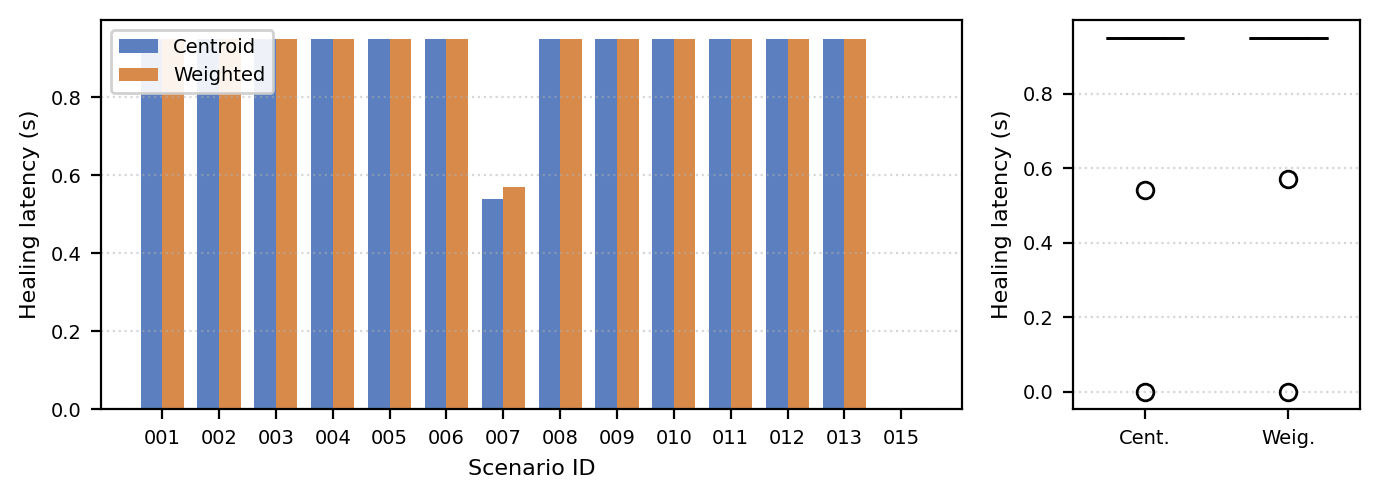
\includegraphics[width=\columnwidth]{latency_distribution.png}
    \caption{Healing-latency distribution across the 15 scenarios. Left:
    per-scenario values for both controllers. Right: aggregate boxplot.}
    \label{fig:latency-dist}
\end{figure}

\subsection{Parameter Sensitivity}
The controller gains $K_{att}=0.3$, $K_{rep}=8.0$, and $D_{safe}=2.0$\,m
were selected by a grid search that, for each candidate triple, scored
oscillation amplitude, time-to-target, and minimum inter-drone distance.
In practice, increasing $K_{att}$ shortens convergence time, but causes 
relay drones to overshoot the midpoint, especially when the velocity cap
$V_{max}$ saturates and the drone cannot decelerate before crossing.
Reducing $K_{att}$ from the previous tested value of $1.0$ to $0.3$ removed
visible oscillations at the cost of about $1$\,s of extra settling
time. In contrast, raising $K_{rep}$ or $D_{safe}$ widens the safety margin, but 
when repulsion dominates attraction, helpers fail to compress
into a relay chain near the boundary, and the lost drone is never bridged.
Drone mass acts like damping through $\mathbf{a}=\mathbf{F}_{tot}/m$:
heavier drones smooth the response but slow convergence. The chosen triple
sits where oscillations are damped, the chain still compresses, and
time-to-target stays bounded.

Figure~\ref{fig:connections_over_time} traces active connections during a
representative run, showing the transition from isolated links to a restored
multi-hop relay.

\begin{figure}[t]
    \centering
    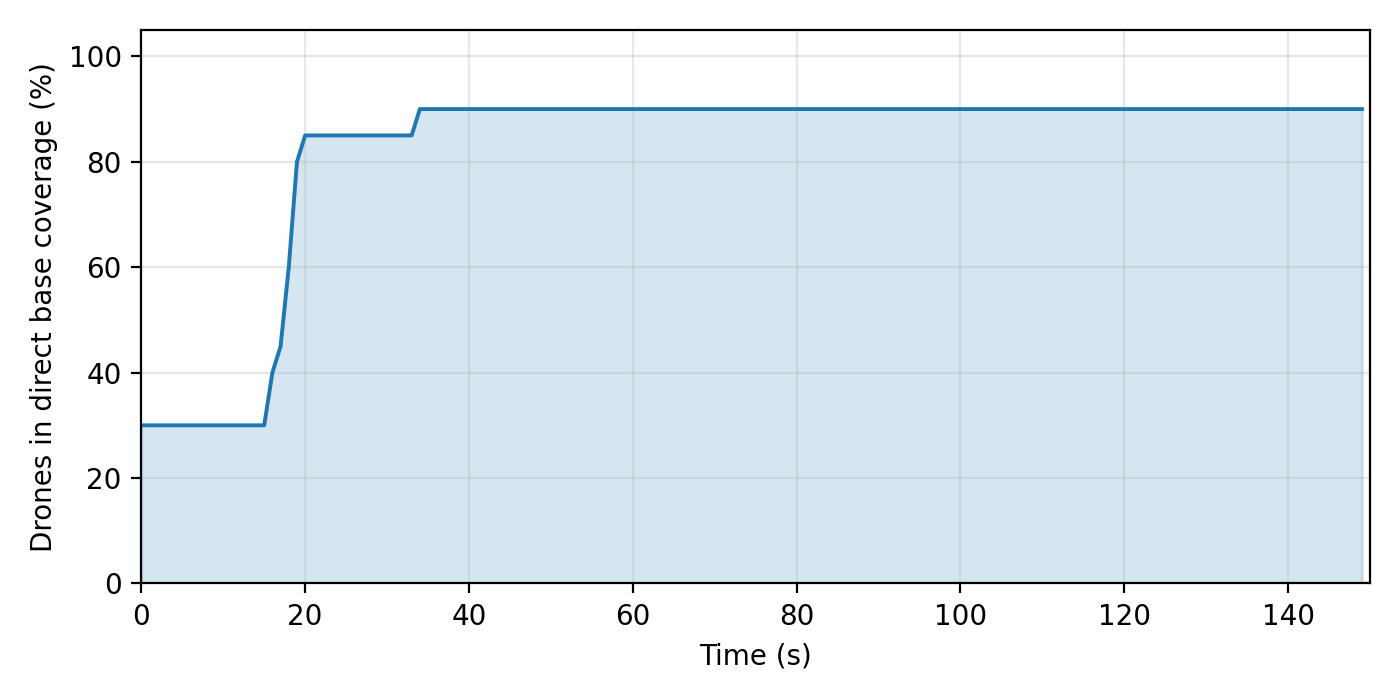
\includegraphics[width=\columnwidth]{connections_over_time.png}
    \caption{Node connections over time in a representative run.}
    \label{fig:connections_over_time}
\end{figure}

\section{Future Work}
\label{sec:future}
This is a work-in-progress and several extensions are planned for the full
version. \textit{Multi-base topologies}: extend the
flooding and neighbor exchange to track per-base hop counts independently
and let each drone optimize against its nearest reachable base.
\textit{Base-station failure tolerance}: add scheduled base kills to the
batch and quantify recovery as drones reattach to surviving bases,
including cascading scenarios where multiple bases fail in sequence.
\textit{Channel realism}: replace the strict range-cutoff UWB model with a
path-loss/fading propagation model.
\textit{Parameter analysis}: report a complete sensitivity sweep over 
$(K_{att},K_{rep},D_{safe})$ rather than the qualitative summary given here, 
including the trade-off between healing latency and station-keeping drift. 
\textit{Network scale}: extend the evaluation beyond 20 drones and include 
heterogeneous swarms with mixed roles. 
\textit{Hardware validation}: port the stack to Crazyflie~2.1 with
Loco UWB anchors and reproduce the baseline scenario in a flying arena to
quantify the sim-to-real gap.

\section{Conclusions}
\label{sec:conclusions}
In this work in progress paper, we presented a decentralized self-healing protocol that combines ACK-based reachability detection, flooding-based hop discovery, neighbor broadcasts, and a virtual spring-damper controller, with GPS-free UWB localization. Across 15 single-base scenarios, the protocol restores connectivity in $\sim1$\,s per scenario; the centroid and weighted variants of the controller are tied on healing latency, while the weighted variant delivers shorter return phases ($-8\%$ mean). 
The comparison under partitioned topologies is left to future work (multi-base and base-failure extensions mentioned in Section~\ref{sec:future}). Limitations include the need for at least one in-range peer for a lost drone, dependence on anchor density for localization,
and a kinematic mobility model that ignores aerodynamics, and multipath.

\bibliographystyle{IEEEtran}
\bibliography{references}

\end{document}
